\paragraph{Architectural decisions} 

Aquarium's architectural design is driven by two requirements: scaling
and fault tolerance. Although initially we used a 3-tiered
architecture, it quickly became clear that it would not meet our
needs. Complications arose from the difficulty of describing versioned
tree-based structures, such as the configuration {\sc dsl}, in a
relational format, and in making sure that resource events were
described in an abstract way that would be adaptable to all future
system expansions. Moreover, for performance reasons, Aquarium must
maintain in-memory caches of computed values; for example the single
query that cloud services will be asking Aquarium continually (number
of remaining credits) must be answered within a few milliseconds for a
large number of concurrent requests. Consequently, Aquarium's data
processing architecture was based on the event sourcing
pattern~\cite{Fowle05}, while system state handling and processing
components are modeled as collections of actors~\cite{Hewit73}.

Event sourcing assumes that all changes to application state are
stored as a sequence of events, in an immutable log. With such a log,
Aquarium can rebuild its state at any point in time by replaying the
events in order, so it is possible to perform queries on past system
states for debugging purposes. Similarly, Aquarium can concurrently
employ several event processing models to cater for different
front-end data requirements. Furthermore, application crashes are not
destructive for Aquarium, as long as event replay is fast enough and
no state is inserted to the application without being recorded to the
event log first.

\begin{figure}
    \begin{center}
    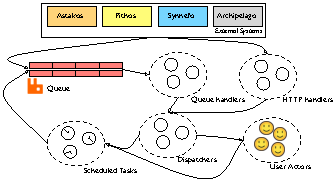
\includegraphics[scale=1.2]{arch.pdf}
    \end{center}
\caption{Functional components in Aquarium's architecture} 
\label{fig:arch}
\end{figure}

We use actors to encapsulate state. The actor model guarantees that
only one thread touches the actor state, thus eliminating the need for
locks.

\paragraph{Components} An overview of the Aquarium architecture is
presented in Figure~\ref{fig:arch}. The system is modeled as a
collection of logically and functionally isolated components that
communicate by message passing. Within each component, a number of
actors take care of concurrently processing incoming messages through
a load balancer component that is the gateway to requests targeted to
the component. Each component is also monitored by its own supervisor;
should an actor fail, the supervisor will automatically restart it.
The architecture allows certain application paths to fail individually
while the system is still responsive, while also enabling future
distribution of multiple components on clusters of machines.

The system receives input mainly from two sources: queues for
resource and user events and a {\sc rest api} for credits and resource
state queries. The queue component reads messages from a configurable
number of queues and persists them in the application's immutable log
store. Both input components then forward incoming messages to a
network of dispatcher handlers which do not do any processing by
themselves, but know where the user actors lay. As described earlier,
actual processing of billing events is done within the user actors.
Finally, a separate network of actors take care of scheduling periodic
tasks, such as refiling of user credits; they do so by issuing events
to the appropriate queue.

\paragraph{Implementation}

Aquarium is being developed as a standalone service, based on the Akka
library for handling actor related functionality. Akka also provided
actor-based components for communicating with the message queue and,
through a third party component (Spray), facilities for handling {\sc
  rest} requests. We chose the {\sc amqp} protocol and its Rabbit{\sc
  mq} implementation for implementing the request queue because recent
versions include support for active/active cluster configurations. The
persistence layer is currently implemented by Mongo{\sc db}, for its
replication and sharding support. However, this is not a hard
requirement, as Aquarium features an abstraction layer for all
database queries (currently 10 methods), which can then be implemented
by any persistence system, relational or not.
